\section{Artifact Contract}
\label{sec:artifacts}

\subsection{Manifests}

Every runner reads a manifest, never a raw dataset CSV. The contract requires \texttt{image\_id} (unique and the resume key), \texttt{image\_relpath}, \texttt{dataset}, \texttt{patient\_id} (the cluster key), and \texttt{split}. Classification manifests carry eight label columns whose cells must be the exact strings \texttt{positive}, \texttt{negative}, or \texttt{unknown}; integers, booleans, and empty strings are contract violations because two independent code paths silently convert them to ``negative'' or drop the finding.

The NIH manifest contains 1,732 rows: 1,054 internal-test, 452 source-val, and 226 internal-train donor rows used to repair \texttt{no\_finding}. The scored set is 1,506. To make that denominator impossible to confuse with the manifest size, the harness writes a split-pure evaluation manifest (1,506 rows) and a SHA-256 lock file with row count, byte size, and digest for every manifest the paper uses. The donor rows remain in the parent manifest; the evaluation path never reads them because every runner passes \texttt{--split internal\_test,source\_val}.

\subsection{Predictions}

Each prediction row is a JSON object with \texttt{image\_id}, \texttt{dataset}, \texttt{split}, \texttt{condition}, \texttt{severity}, \texttt{param}, \texttt{raw\_output}, \texttt{error}, \texttt{elapsed\_sec}, \texttt{parsed}, and \texttt{ground\_truth}. \texttt{parsed} contains the parse status, parse error, and per-label status, probability, and confidence. This single schema is shared by synthetic shift, reliance, precision control, schema ablation, native shift, and report generation; report rows add \texttt{reference\_text} and \texttt{evidence\_method}. A reader can therefore compute a metric without knowing which runner produced the row.

\subsection{Coverage census}

The harness counts, for every model--stage file, rows, parse successes, error rows, structured replies, and all-definite replies (all eight statuses positive or negative). The census is the empirical answer to a question that a results table hides: is a low score caused by wrong answers, or by missing answers? Figure~\ref{fig:coverage} and Table~\ref{tab:coverage} show the answer on the NIH shift grid.

\begin{figure}[t]
\centering
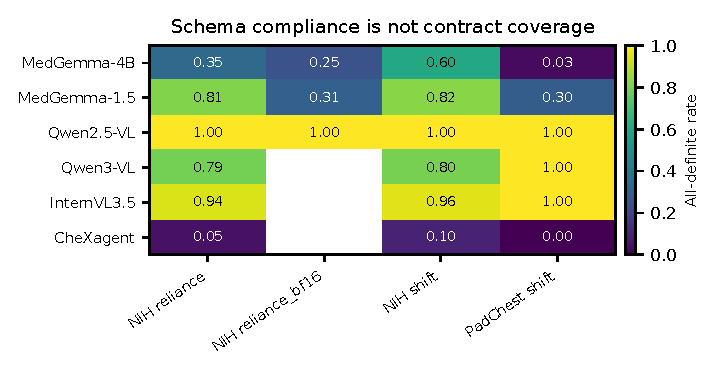
\includegraphics[width=0.86\textwidth]{figures/fig2_coverage.pdf}
\caption{All-definite rate by model and stage. Schema compliance and contract coverage are different quantities: a reply can parse and still leave most label slots \texttt{uncertain} or \texttt{not\_mentioned}. The white cell is a precision control not run for Qwen3-VL (already bf16).}
\label{fig:coverage}
\end{figure}

\begin{table}[t]
\centering
\small
\caption{NIH shift grid coverage (28,614 calls per model). ``All definite'' is the fraction of parsed replies with all eight statuses positive/negative. Every delivered call is a persisted row; the matrix contains no duplicate keys and no lost calls (Section~\ref{sec:evaluation}).}
\label{tab:coverage}
\begin{tabular}{lrrr}
\toprule
Model & Parse rate & All definite & Error rows \\
\midrule
Qwen2.5-VL & 1.000 & \textbf{1.000} & 0 \\
InternVL3.5 & 1.000 & 0.956 & 0 \\
MedGemma-1.5 & 0.998 & 0.824 & 0 \\
Qwen3-VL & 1.000 & 0.795 & 0 \\
MedGemma-4B & 1.000 & 0.605 & 0 \\
CheXagent & 0.985 & \textbf{0.096} & 0 \\
\bottomrule
\end{tabular}
\end{table}

The table explains why a single ``accuracy'' column is insufficient. Qwen2.5-VL parses every reply and makes every slot definite; CheXagent parses 98.5\% but only 9.6\% of parsed replies have all eight statuses definite. The two models are not on the same denominator, and the census makes that visible before any metric is computed.
